%\VignetteEngine{knitr::knitr}
%\VignetteIndexEntry{mixedMem}
\documentclass{article}\usepackage[]{graphicx}\usepackage[]{color}
%% maxwidth is the original width if it is less than linewidth
%% otherwise use linewidth (to make sure the graphics do not exceed the margin)
\makeatletter
\def\maxwidth{ %
  \ifdim\Gin@nat@width>\linewidth
    \linewidth
  \else
    \Gin@nat@width
  \fi
}
\makeatother

\definecolor{fgcolor}{rgb}{0.345, 0.345, 0.345}
\newcommand{\hlnum}[1]{\textcolor[rgb]{0.686,0.059,0.569}{#1}}%
\newcommand{\hlstr}[1]{\textcolor[rgb]{0.192,0.494,0.8}{#1}}%
\newcommand{\hlcom}[1]{\textcolor[rgb]{0.678,0.584,0.686}{\textit{#1}}}%
\newcommand{\hlopt}[1]{\textcolor[rgb]{0,0,0}{#1}}%
\newcommand{\hlstd}[1]{\textcolor[rgb]{0.345,0.345,0.345}{#1}}%
\newcommand{\hlkwa}[1]{\textcolor[rgb]{0.161,0.373,0.58}{\textbf{#1}}}%
\newcommand{\hlkwb}[1]{\textcolor[rgb]{0.69,0.353,0.396}{#1}}%
\newcommand{\hlkwc}[1]{\textcolor[rgb]{0.333,0.667,0.333}{#1}}%
\newcommand{\hlkwd}[1]{\textcolor[rgb]{0.737,0.353,0.396}{\textbf{#1}}}%

\usepackage{framed}
\makeatletter
\newenvironment{kframe}{%
 \def\at@end@of@kframe{}%
 \ifinner\ifhmode%
  \def\at@end@of@kframe{\end{minipage}}%
  \begin{minipage}{\columnwidth}%
 \fi\fi%
 \def\FrameCommand##1{\hskip\@totalleftmargin \hskip-\fboxsep
 \colorbox{shadecolor}{##1}\hskip-\fboxsep
     % There is no \\@totalrightmargin, so:
     \hskip-\linewidth \hskip-\@totalleftmargin \hskip\columnwidth}%
 \MakeFramed {\advance\hsize-\width
   \@totalleftmargin\z@ \linewidth\hsize
   \@setminipage}}%
 {\par\unskip\endMakeFramed%
 \at@end@of@kframe}
\makeatother

\definecolor{shadecolor}{rgb}{.97, .97, .97}
\definecolor{messagecolor}{rgb}{0, 0, 0}
\definecolor{warningcolor}{rgb}{1, 0, 1}
\definecolor{errorcolor}{rgb}{1, 0, 0}
\newenvironment{knitrout}{}{} % an empty environment to be redefined in TeX

\usepackage{alltt}

\linespread{1.6}
\usepackage{amsmath,amsthm,amssymb}
\usepackage[margin = 1in]{geometry} 
\usepackage{natbib, underscore}
\newcommand{\E}{\mathbb{E}}
\usepackage{setspace} 
\renewenvironment{knitrout}{\begin{singlespace}}{\end{singlespace}}
\IfFileExists{upquote.sty}{\usepackage{upquote}}{}
\begin{document}
\title{Fitting Mixed Membership Models using \texttt{mixedMem}\footnotetext{Special thanks to McKay Curtis, Maryclare Griffin and Kevin Lin for providing feedback on package features and usability}}
\author{Y. Samuel Wang and Elena A. Erosheva}
\maketitle

\small
\begin{abstract}
This vignette is a tutorial for the \texttt{mixedMem} R package that allows users to fit and visualize results for a broad class of mixed membership models as specified by \cite{erosheva2004mixed}. Relevant data structures include multivariate outcome vectors. Mixed distribution types and replicate measurements are supported. Version 1.1.0 allows for binary, multinomial or Plackett-Luce rank distribution types. The extended GoM model from \cite{erosheva2007describing} is also supported. This tutorial provides an outline of functions available in the package and a step-by-step guide for fitting mixed membership models. As an example, we carry out a mixed membership analysis to identify latent ideology blocs using political survey data from the 1983 American National Election Survey Pilot.  
\end{abstract}

\normalsize
\section{Mixed Membership Modeling} \label{MMM}
\subsection{Mixed Membership Background}
Mixed membership models provide a useful framework for analyzing multivariate data from heterogeneous populations \citep{Airoldi2014Handbook}. Similar to mixture models, mixed membership models assume that the overall population is comprised of several latent sub-populations or groups. Mixture models, however, assume that each individual within the population belongs to a single group, whereas mixed membership models allow for an individual to belong to multiple groups simultaneously and explicitly specify an individual's degree of membership in each group.

Mixed membership models have been used to analyze to a wide variety of data types. For example, mixed membership analysis of text data \citep{LDA, erosheva2004mixed} can illustrate the latent structure of topics/subjects within a body of documents; analysis of genotype sequences \citep{pritchard2000inference} can describe individuals sharing ancestry across various origin populations; analysis of survey data \citep{erosheva2007describing, grossManriqueVallier} can show how survey respondents belong to various sub-populations; and analysis of ranked votes \citep{gormley2009grade} can characterize latent voting blocs and voting tendencies. The \texttt{mixedMem} package allows for fitting these specific cases of mixed membership models as well as their extensions, using a general framework described by \cite{erosheva2004mixed} with the estimation carried out via a variational EM algorithm.

The remainder of section \ref{MMM} introduces notation and formally defines the generative hierarchy assumed for discrete mixed membership models. Section \ref{variational} outlines the variational EM  method used by the \texttt{mixedMem} package and discusses some of the benefits and drawbacks of the variational approach. Section \ref{politicalSurvey} provides a step-by-step guide for fitting mixed membership models using \texttt{mixedMem}. For illustration, we analyze the results of the 1983 American National Election Studies Pilot Study. Finally, section \ref{conclusion} provides a brief conclusion.

\subsection{Illustration and Notation}
For a hypothetical example, consider a survey of Total =  100 (the number of individuals) high school students with J = 3 (the number of variables) questions. Each individual is asked to (1) rank their favorite classes (rank data), (2) select their favorite TV channel (multinomial data) and (3) indicate whether or not they are on the honor roll (Bernoulli data). Students within the same extracurricular activities/clubs might give similar responses, so in a mixed membership analysis, the latent sub-populations might map to extracurricular groupings. For concreteness, assume the following K = 4 sub-populations fully describe the students' extracurricular activities: athletics, math/science, fine arts and student government. Athletes might be more likely to rank ``Anatomy" and ``Health" among their favorite classes, while students involved in student government might be more likely to rank ``Civics" or ``History" highly.  As is often the case, students may be involved with multiple clubs/activities to varying degrees. If a student is involved in student government and athletics, they might rank their favorite classes as (1. ``Anatomy", 2. ``History" and 3. ``Health"). Thus, using a mixture model framework to classify the student solely as an athlete would fail to represent her full profile. We use $\lambda_i$ to denote the distribution of membership for individual i. $\lambda_i$ is a vector of K non-negative elements which sum to 1. The membership vector $\lambda$ for the student above might be $\left(\text{athletics} = 0.7, \text{math/science} = 0.0, \text{fine arts} = 0.0, \text{student government} = 0.3\right)$. In this package, we assume that memberships are drawn from a Dirichlet distribution; however, some other mixed membership models assume more general distributions for the membership vectors \citep{blei2006correlated}.

We index each of the Total students by $i = 1,2, \ldots Total$; in this case Total = 100. Each of the J variables are indexed by $j = 1,2,\ldots J$ and for each variable we index the $R_j$ number of replicates by $r = 1,2,\ldots R_j$. Note that each of the variables can have a different number of replications. For rank data, we index the $N_{i,j,r}$ ranking levels (ie the first preference, the second preference, ...) by $n = 1,2\ldots N_{i,j,r}$; for multinomial and binary data $N_{i,j,r} = 1$. For each individual i, variable j, replicate r, and ranking level n we denote the observed response by $X_{i,j,r,n}$. For example, if student 10's favorite classes (variable 1)  are $ \left(\text{``Anatomy", ``History", ``Health"}\right)$ and she is on the honor roll (variable 3), then $X_{i = 10,j = 1,r = 1,n = 2} =$ ``History" and  $X_{i = 10,j = 3,r = 1,n = 1} = 1$.    

\subsection{Generative Process}\label{generative}
More formally, for K sub-populations, we assume a mixed membership generative process as follows:

\noindent
For each individual $i = 1,\ldots Total$: Draw $\lambda_i$ from a Dirichlet($\alpha$). $\lambda_i$ is a vector of length K which indicates the degree of membership for individual i.
  \begin{itemize}
  \item For each variable $j = 1, \ldots, J$, each replicate $r = 1, \dots, R_j$ and each ranking level $n = 1\ldots, N_{i,j,r}$: Draw $Z_{i,j,r,n}$ from a multinomial(1, $\lambda_i$). $Z_{i,j,r,n}$ determines the sub-population which governs the response for observation $X_{i,j,r,n}$. This is sometimes referred to as a context vector because it determines the context from which the individual responds.
  \item For each variable $j = 1, \ldots, J$, each replicate $r = 1, \dots, R_j$ and each ranking level $n = 1\ldots, N_{i,j,r}$: Draw $X_{i,j,r,n}$ from the distribution parameterized by $\theta_{j,Z_{i,j,r,n}}$. Here, $\theta$ is the set of parameters which govern the observations for each sub-population. If variable j is a multinomial or rank distribution with $V_j$ categories/candidates, $\theta_{j,k}$ is a vector of length $V_j$ which parameterizes the responses to variable j for sub-population k. If variable j is a Bernoulli random variable, then $\theta_{j,k}$ is a value which determines the probability of success. 
  \end{itemize}
  
In topic models, \cite{LDA, erosheva2004mixed} analyze individual articles; the latent sub-populations are topics for each of the articles; the the observed words are draws from a multinomial distribution determined by the topic; and we observe many replicates (words) for each article . In the analysis of genotype sequences, \cite{pritchard2000inference} analyze individuals; the latent sub-populations map to genetically similar groups; each observed genetic loci is a different variable; and there are two replicates (assuming diploid individuals) for each variable. In the analysis of ranked votes, \cite{gormley2009grade} analyze individual voters; the latent sub-populations map to voting blocs; the observed data the a list of candidates by preference for each individual; and the ranking levels ($N_{ijr}$) for each individual is the number of candidates they list.     

\section{Variational EM and the \texttt{mixedMem} Package}\label{variational}

\subsection{Fitting Mixed Membership Models}
When using a mixed membership model, the interest is typically in estimating the sub-population parameters $\theta$, the Dirichlet parameter $\alpha$ and the latent memberships of individuals $\lambda$. Estimation of these quantities through maximum likelihood or direct posterior inference is computationally intractable in a mixed membership model, so Markov Chain Monte Carlo or variational inference techniques are used instead \citep{airoldi2009mixed}. Most MCMC analyses typically require large amounts of human effort to tune and check the samplers for convergence. Furthermore, in mixed membership models, we must sample a latent membership for each individual and a context vector for each observed response; thus, a mixed membership MCMC analysis becomes very computationally expensive as the number of individuals grows. \texttt{mixedMem} circumvents these difficulties by employing a variational EM algorithm which is a deterministic and computationally attractive alternative for fitting mixed membership models. Using a variational approach allows us to fit larger models and avoids tedious human effort by approximating the true posterior and replacing the MCMC sampling procedure with an optimization problem \citep{beal2003variational}.  

\subsection{Variational EM}\label{VI}
To fit a mixed membership model, the variational EM algorithm combines variational inference (inference on an approximate posterior) to estimate the group memberships $\lambda$ and a pseudo maximum likelihood procedure to estimate the group parameters $\theta$ and Dirichlet parameter $\alpha$.

Instead of working with the intractable true posterior, variational inference employs a more computationally tractable approximate variational distribution. This variational distribution, denoted by Q, is parameterized by $\phi$ and $\delta$ as follows: 

\begin{equation} \label{eq:varDist}
p(\lambda, Z|X) \approx Q(\lambda,Z|\phi, \delta) = \prod_i^T \text{Dirichlet}(\lambda_i|\phi_i)\prod_j^J \prod_r^{R_j} \prod_n^{N_{i,j,r}}\text{multinomial}(Z_{i,j,r,n}|\delta_{i,j,r,n}).
\end{equation}

The parameters $\phi$ and $\delta$ can be selected to minimize the Kullback-Leibler divergence between the true posterior distribution and the variational distribution Q \citep{beal2003variational}. This provides an approximate distribution which can be used to carry out posterior inference on the latent variables and posterior means which can be used as point estimates for $\lambda$.

This variational distribution can also be used in an alternative pseudo-likelihood framework, to select the global parameters $\theta$ and $\alpha$. Using Jensen's inequality, the variational distribution can be used to derive a function of $\phi$, $\delta$, $\alpha$ and $\theta$ which is a lower bound on the log-likelihood of our observations:

\begin{equation}\label{eq:Jensen}
\log\left[p(X|\alpha, \theta)\right] \geq \E_Q\left\{\log\left[p(X,Z, \Lambda)\right]\right\} - \E_Q\left[\log\left[Q(Z, \Lambda|\phi, \delta)\right]\right\}.
\end{equation}

The lower bound on the RHS of equation (\ref{eq:Jensen}) is often called the ELBO for \textbf{E}vidence \textbf{L}ower \textbf{Bo}und. Calculating the LHS of equation (\ref{eq:Jensen}) is intractable, but for a fixed $\phi$ and $\delta$, selecting $\alpha$ and $\theta$ to maximize the lower bound on the RHS is a tractable alternative to maximum likelihood estimation. 

It can be shown that minimizing the KL Divergence between Q and the true posterior is actually equivalent to maximizing the lower bound in equation (\ref{eq:Jensen}) with respect to $\phi$ and $\delta$ \citep{beal2003variational}. Thus, the tasks of finding an approximate posterior distribution with respect to $\phi$ and $\delta$ and picking pseudo-MLE's $\theta$ and $\alpha$ are both achieved by maximizing the lower bound in equation (\ref{eq:Jensen}). In practice, we maximize this lower bound through a variational EM procedure. In the E-step (variational inference), we fix $\theta$ and $\alpha$ and minimize the KL divergence between Q and the true posterior   (this is also equivalent to maximizing the lower bound in equation (\ref{eq:Jensen}) through iterative closed form updates to $\phi$ and $\delta$. In the M-step (pseudo-MLE), we fix $\phi$ and $\delta$ and select the $\theta$ and $\alpha$ which maximize the lower bound through gradient based methods. The entire procedure iterates between the E-step and the M-step until reaching a local mode. A detailed exposition of variational inference is provided by \cite{jaakkola200110}.

\subsubsection{Label Switching in Mixed Membership Models}
Mixed membership models are only identifiable up to permutations of the sub-population labels (ie simultaneously permuting the labels for all group memberships and distribution parameters). In an MCMC analysis of mixed membership models, this can require special attention if label switching is present within a sampler \citep{stephens2000dealing}. Because variational EM is a deterministic approach, the final permutation of the labels is only dependent on the initialization points and does not require special attention during the fitting procedure. However matching group labels can still a concern for assessing model fit when comparing to some other fitted model. \texttt{mixedMem} provides functions discussed in subsection \ref{postProcess}  for dealing with the label permutations to facilitate post-processing.   

\subsubsection{Variational EM Caveats}
The computational benefits of variational EM, however, do not come for free. The lower bound in equation (\ref{eq:Jensen}), is generally not a strictly convex function, so only convergence to a local mode, not the global mode, is guaranteed \citep{wainwright2008graphical}. If prior knowledge exists about a specific problem, initializing $\theta$ and $\alpha$ near plausible values is helpful in ensuring that the EM algorithm reaches a reasonable mode. In general though, starting from multiple initialization points and selecting the mode with the largest ELBO is highly recommended. This is also an area where the post-processing tools discussed in subsection \ref{postProcess} can be useful for determining if candidate modes found from different initialization points are conceptually different.

Variational inference also lacks any guarantees on the quality of our approximation. In some cases, we anecdotally find that the estimates of $\alpha$ provide good estimates of relative frequency, but can inaccurately estimate the rate of intra-individual dispersion (which is regulated by $\sum \alpha_i$). However, \cite{erosheva2007describing} show that a mixed membership analysis of survey data using a MCMC and variational approach agree well, and, in practice, we see that variational inference provides reasonable and interpretable results in mixed membership models \citep{LDA, erosheva2004mixed, airoldi2009mixed}. However, there are no theoretical guarantees on how good or bad our approximation ultimately is.

\section{Example: Fitting Political Survey Data with \texttt{mixedMem}} \label{politicalSurvey}
For demonstration, we present a \texttt{mixedMem} analysis of political opinion survey data previously analyzed by  \cite{grossManriqueVallier} as well as \cite{feldman1988structure}. Within this context, identified latent sub-populations might map to ideological blocs. Since individuals often hold to political ideologies to varying degrees, a mixed membership model is particularly appropriate. We utilize the mixed membership model as specified by Gross and Manrique-Vallier and discussed more generally in section \ref{generative}. The model assumes 3 latent sub-populations (K = 3) with 19 observed multinomial variables with 1 replicate each. Gross and Manrique-Vallier specify a fully Bayesian approach, placing prior distributions on both $\theta$ and $\alpha$ and utilize MCMC to estimate the model. This allows for posterior inference on both the latent memberships as well as on $\theta$ and $\alpha$. Our analysis using \texttt{mixedMem} will fit the model using the variational EM algorithm  which allows for posterior inference on $\lambda$ and Z, but only yields point estimates for $\alpha$ and $\theta$. Nonetheless, we will show that the two methods yield comparable results with very similar interpretations.

In the 1983 American National Election Survey Pilot \citep{ANES}, each individual was prompted with various opinion-based statements and was asked to report their agreement with the statement using the categories: ``strongly agree", ``agree but not strongly", ``can't decide", ``disagree but not strongly", and ``strongly disagree". For example, one statement was ``Any person who is willing to work hard has a good chance of succeeding". We specifically study 19 of the statements which were selected by \cite{feldman1988structure} and reanalyzed by \citep{grossManriqueVallier}.  The 19 statements can be grouped into 3 overarching themes: Equality (abbreviated ``EQ" in the data set variable names), Economic Individualism (abbreviated ``IND") and Free Enterprise (abbreviated ``ENT") \citep{feldman1988structure}.  Following the original analysis of \cite{grossManriqueVallier}, we include the 279 complete responses and combine categories ``agree" with ``strongly agree" and ``disagree"  with ``strongly disagree", leaving the 3 possible responses ``agree" = 0, ``can't decide" = 1, and ``disagree" = 2 to avoid overparameterization. The data is included in \texttt{mixedMem} as \texttt{ANES}; the full text statement for each variable can be accessed through \texttt{help(ANES)}. 

A brief exploratory analysis, shows that of the $279 \times 19 = 5301$ total responses, 3295 responses are ``agree" 1907 are ``disagree" and only 99 are ``can't decide".



\begin{knitrout}
\definecolor{shadecolor}{rgb}{0.969, 0.969, 0.969}\color{fgcolor}\begin{kframe}
\begin{alltt}
\hlkwd{library}\hlstd{(mixedMem)}
\hlkwd{data}\hlstd{(ANES)}
\hlcom{# Dimensions of the data set: 279 individuals with 19 responses each}
\hlkwd{dim}\hlstd{(ANES)}
\end{alltt}
\begin{verbatim}
## [1] 279  19
\end{verbatim}
\begin{alltt}
\hlcom{# The 19 variables and their categories}
\hlcom{# The specific statements for each variable can be found using help(ANES)}
\hlcom{# Variables titled EQ are about Equality}
\hlcom{# Variables titled IND are about Econonic Individualism}
\hlcom{# Variables titled ENT are about Free Enterprise}
\hlkwd{colnames}\hlstd{(ANES)}
\end{alltt}
\begin{verbatim}
##  [1] "EQ1"  "EQ2"  "EQ3"  "EQ4"  "EQ5"  "EQ6"  "EQ7"  "IND1" "IND2" "IND3"
## [11] "IND4" "IND5" "IND6" "ENT1" "ENT2" "ENT3" "ENT4" "ENT5" "ENT6"
\end{verbatim}
\begin{alltt}
\hlcom{# Distribution of responses}
\hlkwd{table}\hlstd{(}\hlkwd{unlist}\hlstd{(ANES))}
\end{alltt}
\begin{verbatim}
## 
##    0    1    2 
## 3295   99 1907
\end{verbatim}
\end{kframe}
\end{knitrout}

\subsection{Step 1: Initializing the \texttt{mixedMemModel} Object}
To fit a mixed membership model, we must first initialize a \texttt{mixedMemModel} object using the class constructor. The \texttt{mixedMemModel} object contains the dimensions of our mixed membership model, the observed data and initialization points for $\alpha$ and $\theta$. Creating a \texttt{mixedMemModel} object provides a vehicle for passing this information to the \texttt{mmVarFit} function in step 2. This is similar to how one might specify the formula for an \texttt{lm} object. Although initialization points for $\phi$ and $\delta$ can be passed to the constructor as well, these by default are initialized uniformly across the sub-populations, and unless there is very strong prior knowledge, we recommend that the default values be used. For this particular model, all the variables are multinomials; an example showing an initialization of mixed data types can be accessed through \texttt{help(mixedMemModel)}.

As mentioned previously, because the lower bound function is not convex, different initializations may result in convergence to different local modes. After initializing at various point, we found that the initialization of $\alpha = \left(.2, .2, .2\right)$ and $\theta \sim \text{Dirichlet}(.8)$ using seed 123 resulted in the highest lower bound at convergence.  

\begin{knitrout}
\definecolor{shadecolor}{rgb}{0.969, 0.969, 0.969}\color{fgcolor}\begin{kframe}
\begin{alltt}
\hlcom{# Sample Size}
\hlstd{Total} \hlkwb{<-} \hlnum{279}
\hlcom{# Number of variables}
\hlstd{J} \hlkwb{<-} \hlnum{19}
\hlcom{# we only have one replicate for each of the variables}
\hlstd{Rj} \hlkwb{<-} \hlkwd{rep}\hlstd{(}\hlnum{1}\hlstd{, J)}
\hlcom{# Nijr indicates the number of ranking levels for each variable.}
\hlcom{# Since all our data is multinomial it should be an array of all 1s}
\hlstd{Nijr} \hlkwb{<-} \hlkwd{array}\hlstd{(}\hlnum{1}\hlstd{,} \hlkwc{dim} \hlstd{=} \hlkwd{c}\hlstd{(Total, J,} \hlkwd{max}\hlstd{(Rj)))}
\hlcom{# Number of sub-populations}
\hlstd{K} \hlkwb{<-} \hlnum{3}
\hlcom{# There are 3 choices for each of the variables ranging from 0 to 2.}
\hlstd{Vj} \hlkwb{<-} \hlkwd{rep}\hlstd{(}\hlnum{3}\hlstd{, J)}
\hlcom{# we initialize alpha to .2}
\hlstd{alpha} \hlkwb{<-} \hlkwd{rep}\hlstd{(}\hlnum{.2}\hlstd{, K)}
\hlcom{# All variables are multinomial}
\hlstd{dist} \hlkwb{<-} \hlkwd{rep}\hlstd{(}\hlstr{"multinomial"}\hlstd{, J)}
\hlcom{# obs are the observed responses. it is a 4-d array indexed by i,j,r,n}
\hlcom{# note that obs ranges from 0 to 2 for each response}
\hlstd{obs} \hlkwb{<-} \hlkwd{array}\hlstd{(}\hlnum{0}\hlstd{,} \hlkwc{dim} \hlstd{=} \hlkwd{c}\hlstd{(Total, J,} \hlkwd{max}\hlstd{(Rj),} \hlkwd{max}\hlstd{(Nijr)))}
\hlstd{obs[, ,} \hlnum{1}\hlstd{,} \hlnum{1}\hlstd{]} \hlkwb{<-} \hlkwd{as.matrix}\hlstd{(ANES)}

\hlcom{# Initialize theta randomly with Dirichlet distributions}
\hlkwd{set.seed}\hlstd{(}\hlnum{123}\hlstd{)}
\hlstd{theta} \hlkwb{<-} \hlkwd{array}\hlstd{(}\hlnum{0}\hlstd{,} \hlkwc{dim} \hlstd{=} \hlkwd{c}\hlstd{(J, K,} \hlkwd{max}\hlstd{(Vj)))}
\hlkwa{for} \hlstd{(j} \hlkwa{in} \hlnum{1}\hlopt{:}\hlstd{J) \{}
    \hlstd{theta[j, , ]} \hlkwb{<-} \hlstd{gtools}\hlopt{::}\hlkwd{rdirichlet}\hlstd{(K,} \hlkwd{rep}\hlstd{(}\hlnum{.8}\hlstd{, Vj[j]))}
\hlstd{\}}

\hlcom{# Create the mixedMemModel}
\hlcom{# This object encodes the initialization points for the variational EM algorithim}
\hlcom{# and also encodes the observed parameters and responses}
\hlstd{initial} \hlkwb{<-} \hlkwd{mixedMemModel}\hlstd{(}\hlkwc{Total} \hlstd{= Total,} \hlkwc{J} \hlstd{= J,} \hlkwc{Rj} \hlstd{= Rj,}
                         \hlkwc{Nijr} \hlstd{= Nijr,} \hlkwc{K} \hlstd{= K,} \hlkwc{Vj} \hlstd{= Vj,} \hlkwc{alpha} \hlstd{= alpha,}
                         \hlkwc{theta} \hlstd{= theta,} \hlkwc{dist} \hlstd{= dist,} \hlkwc{obs} \hlstd{= obs)}
\end{alltt}
\end{kframe}
\end{knitrout}

\subsection{Step 2: Fitting the Model}
Now we can fit the model using the \texttt{mmVarFit} function. When we call \texttt{mmVarFit}, the function first checks for internal consistency in the input model, \texttt{initial} (i.e., it checks whether the dimensions of the observation match the specified number of variables, etc). If the model check passes, the function begins to iterate through the E-step and M-step described in subsection \ref{VI}. When the algorithm converges, \texttt{mmVarFit} prints the value of the lower bound at convergence as well as the number of EM iterations needed for convergence.

\begin{knitrout}
\definecolor{shadecolor}{rgb}{0.969, 0.969, 0.969}\color{fgcolor}\begin{kframe}
\begin{alltt}
\hlkwd{computeELBO}\hlstd{(initial)}
\end{alltt}
\begin{verbatim}
## [1] -16810.18
\end{verbatim}
\begin{alltt}
\hlstd{st} \hlkwb{=} \hlkwd{proc.time}\hlstd{()}
\hlcom{#printStatus 1 indicates that status updates will be printed}
\hlcom{# printMod 25 indicates that status updates will only be printed ever 25th step}
\hlstd{out} \hlkwb{<-} \hlkwd{mmVarFit}\hlstd{(initial,} \hlkwc{printStatus} \hlstd{=} \hlnum{1}\hlstd{,} \hlkwc{printMod} \hlstd{=} \hlnum{25}\hlstd{)}
\end{alltt}
\begin{verbatim}
## [1] "Model Check: Ok!"
## [1] "<== Beginning Model Fit! ==>"
## Iter: 25 Elbo: -3138.87
## E-Step: -3138.28
## M-Step: -3137.71
## Iter: 50 Elbo: -3125.55
## E-Step: -3125.45
## M-Step: -3125.36
## Iter: 75 Elbo: -3123.26
## E-Step: -3123.24
## M-Step: -3123.22
## Iter: 100 Elbo: -3122.9
## E-Step: -3122.9
## M-Step: -3122.9
## Fit Complete! Elbo: -3122.89 Iter: 103
\end{verbatim}
\begin{alltt}
\hlstd{end} \hlkwb{<-} \hlkwd{proc.time}\hlstd{()}
\hlkwd{computeELBO}\hlstd{(out)}
\end{alltt}
\begin{verbatim}
## [1] -3122.886
\end{verbatim}
\begin{alltt}
\hlstd{time} \hlkwb{<-} \hlstd{end} \hlopt{-} \hlstd{st}
\end{alltt}
\end{kframe}
\end{knitrout}

Notice that the lower bound (our objective function) is \ensuremath{-1.681018\times 10^{4}} at the initialized points and is \ensuremath{-3122.89} at convergence. On a laptop (quad-core 2.4 GHZ with 12 GB of RAM), fitting the entire model took only 10.84 seconds, significantly faster than a full MCMC analysis. 

We can also view a quick summary of the fit model using the \texttt{summary} function.

\begin{knitrout}
\definecolor{shadecolor}{rgb}{0.969, 0.969, 0.969}\color{fgcolor}\begin{kframe}
\begin{alltt}
\hlkwd{summary}\hlstd{(out)}
\end{alltt}
\begin{verbatim}
## == Summary for Mixed Membership Model ==
## Total: 279		 K: 3		 ELBO: -3122.89
## 
##  Variable   Variable Type     Replicates     Categories  
##    1        multinomial       1              3           
##    2        multinomial       1              3           
##    3        multinomial       1              3           
##    4        multinomial       1              3           
##    5        multinomial       1              3           
##    6        multinomial       1              3           
##    7        multinomial       1              3           
##    8        multinomial       1              3           
##    9        multinomial       1              3           
##    10       multinomial       1              3           
##    11       multinomial       1              3           
##    12       multinomial       1              3           
##    13       multinomial       1              3           
##    14       multinomial       1              3           
##    15       multinomial       1              3           
##    16       multinomial       1              3           
##    17       multinomial       1              3           
##    18       multinomial       1              3           
##    19       multinomial       1              3
\end{verbatim}
\end{kframe}
\end{knitrout}

\subsection{Step 3: Post-Processing} \label{postProcess}
In many cases, we may be interested in comparing our fitted model to some ground truth or comparing various runs with different starting values. Since the model is invariant to label permutations, we use the \texttt{findLabels} function to match our sub-population labels to the ground truth labels to facilitate comparison. In this case, we are interested in comparing our fitted values with the posterior means from the original MCMC analysis of \cite{grossManriqueVallier}. The \texttt{findLabels} function finds the permutation of labels which minimizes the weighted squared error shown in equation (\ref{eq:loss}). Once we have found the optimal permutation, we then permute the sub-population labels using the \texttt{permuteLabels} function. 

\begin{equation}\label{eq:loss}
Loss = \sum_i^{T} \sum_j^J \frac{\hat \alpha_k}{\hat \alpha_0} \sum_v^{V_j}(\hat \theta_{j,k,v} - \theta_{j,k,v})^2
\end{equation}

Where $\hat \alpha_0 = \sum_k \alpha_k$.

\begin{knitrout}
\definecolor{shadecolor}{rgb}{0.969, 0.969, 0.969}\color{fgcolor}\begin{kframe}
\begin{alltt}
\hlcom{#read in GM estimates}
\hlcom{# Note that Gross and Manrique-Vallier do not report estimates for the third group, so they have been set to 0 in the data}
\hlkwd{data}\hlstd{(gmv_theta)}
\hlcom{#}
\hlstd{optimal.perm} \hlkwb{<-} \hlkwd{findLabels}\hlstd{(out, gmv_theta)}
\hlcom{# display the permutation as well as the weighted squared error loss}
\hlstd{optimal.perm}
\end{alltt}
\begin{verbatim}
## $perm
## [1] 3 2 1
## 
## $loss
## [1] 7.398825
\end{verbatim}
\begin{alltt}
\hlcom{# save object with permuted labels}
\hlstd{out.permute} \hlkwb{<-} \hlkwd{permuteLabels}\hlstd{(out, optimal.perm}\hlopt{$}\hlstd{perm)}
\end{alltt}
\end{kframe}
\end{knitrout}

\subsection{Step 4: Model Evaluation}
In order to evaluate the goodness of fit for our estimated values of $\theta$ and $\alpha$,
we can calculate a $\chi^2$ statistic by comparing the expected responses from our fitted model to the observed counts. Since the total number of responses for each variable is fixed, this yields a $\chi^2$ statistic with $3 \times (19-1)$ degrees of freedom. 
\begin{knitrout}
\definecolor{shadecolor}{rgb}{0.969, 0.969, 0.969}\color{fgcolor}\begin{kframe}
\begin{alltt}
\hlcom{# calculate the expected value}
\hlstd{model.exp} \hlkwb{<-} \hlkwd{matrix}\hlstd{(}\hlnum{0}\hlstd{,} \hlkwc{nrow} \hlstd{= J,} \hlkwc{ncol} \hlstd{=} \hlkwd{max}\hlstd{(Vj))}
\hlkwa{for}\hlstd{(j} \hlkwa{in} \hlnum{1}\hlopt{:}\hlstd{J)\{}
  \hlstd{model.exp[j, ]} \hlkwb{<-} \hlstd{(out.permute}\hlopt{$}\hlstd{alpha} \hlopt{/} \hlkwd{sum}\hlstd{(out.permute}\hlopt{$}\hlstd{alpha))} \hlopt \hlstd{out.permute}\hlopt{$}\hlstd{theta[j, , ]}
\hlstd{\}}
\hlstd{model.exp} \hlkwb{<-} \hlstd{model.exp}\hlopt{*}\hlstd{out.permute}\hlopt{$}\hlstd{Total}

\hlcom{# aggregate the observed counts}
\hlstd{obs.counts} \hlkwb{<-} \hlkwd{t}\hlstd{(}\hlkwd{apply}\hlstd{(obs[, ,} \hlnum{1}\hlstd{,} \hlnum{1}\hlstd{]} \hlopt{+} \hlnum{1}\hlstd{,} \hlkwc{MARGIN} \hlstd{=} \hlnum{2}\hlstd{, tabulate))}
\hlstd{chi.squared} \hlkwb{<-} \hlkwd{sum}\hlstd{( (obs.counts} \hlopt{-} \hlstd{model.exp)}\hlopt{^}\hlnum{2} \hlopt{/} \hlstd{model.exp)}
\end{alltt}
\end{kframe}
\end{knitrout}

% latex table generated in R 3.1.2 by xtable 1.7-4 package
% Sun Aug 16 14:52:15 2015
\begin{table}[ht]
\centering
\begin{tabular}{rrrrrrr}
  \hline
 & Exp Agree & Obs Agree & Exp Can't Decide & Obs Can't Decide & Exp Disagree & Obs Disagree \\ 
  \hline
EQ1 & 206.7 & 209.0 & 0.7 & 2.0 & 71.5 & 68.0 \\ 
  EQ2 & 61.1 & 60.0 & 10.9 & 13.0 & 207.0 & 206.0 \\ 
  EQ3 & 241.0 & 241.0 & 0.5 & 1.0 & 37.5 & 37.0 \\ 
  EQ4 & 234.4 & 234.0 & 2.2 & 3.0 & 42.4 & 42.0 \\ 
  EQ5 & 257.2 & 255.0 & 0.9 & 3.0 & 20.9 & 21.0 \\ 
  EQ6 & 250.4 & 249.0 & 0.8 & 2.0 & 27.8 & 28.0 \\ 
  EQ7 & 138.1 & 150.0 & 3.4 & 5.0 & 137.6 & 124.0 \\ 
  IND1 & 221.1 & 224.0 & 0.0 & 0.0 & 57.9 & 55.0 \\ 
  IND2 & 74.2 & 72.0 & 1.9 & 3.0 & 202.8 & 204.0 \\ 
  IND3 & 143.9 & 156.0 & 7.1 & 7.0 & 128.0 & 116.0 \\ 
  IND4 & 227.3 & 227.0 & 2.6 & 3.0 & 49.1 & 49.0 \\ 
  IND5 & 140.9 & 134.0 & 1.5 & 2.0 & 136.6 & 143.0 \\ 
  IND6 & 234.5 & 235.0 & 0.5 & 1.0 & 44.0 & 43.0 \\ 
  ENT1 & 185.2 & 188.0 & 5.8 & 9.0 & 88.0 & 82.0 \\ 
  ENT2 & 194.9 & 196.0 & 10.9 & 12.0 & 73.2 & 71.0 \\ 
  ENT3 & 72.1 & 69.0 & 3.3 & 7.0 & 203.6 & 203.0 \\ 
  ENT4 & 108.8 & 105.0 & 7.2 & 11.0 & 163.0 & 163.0 \\ 
  ENT5 & 228.3 & 227.0 & 1.1 & 5.0 & 49.6 & 47.0 \\ 
  ENT6 & 67.0 & 64.0 & 5.3 & 10.0 & 206.7 & 205.0 \\ 
   \hline
\end{tabular}
\caption{Expected responses based on fitted parameters and Observed responses} 
\end{table}


Using this $\chi^2$ statistic, we calculate a p-value of 0.194, which would lead us to fail to reject the null hypothesis that the observed data was generated by the fitted model.  
\begin{knitrout}
\definecolor{shadecolor}{rgb}{0.969, 0.969, 0.969}\color{fgcolor}\begin{kframe}
\begin{alltt}
\hlcom{# The chi squared statistic}
\hlstd{chi.squared}
\end{alltt}
\begin{verbatim}
## [1] 44.93294
\end{verbatim}
\begin{alltt}
\hlcom{# p-value}
\hlkwd{pchisq}\hlstd{(chi.squared,} \hlkwc{df} \hlstd{= (J}\hlopt{-}\hlnum{1}\hlstd{)} \hlopt{*} \hlkwd{max}\hlstd{(Vj))}
\end{alltt}
\begin{verbatim}
## [1] 0.1944583
\end{verbatim}
\end{kframe}
\end{knitrout}


\subsection{Step 4: Interpretation}
Visualizations of the fitted model can be highly context-specific and each of the estimated quantities can be extracted from the output model for further analysis tailored to the scientific question of interest. In the following subsections, we show a few visualizations and tools which may be of general interest.

\begin{knitrout}
\definecolor{shadecolor}{rgb}{0.969, 0.969, 0.969}\color{fgcolor}\begin{kframe}
\begin{alltt}
\hlcom{# The estimated quantities can be exctracted from the output model}
\hlkwd{names}\hlstd{(out)}
\end{alltt}
\begin{verbatim}
##  [1] "Total" "J"     "Rj"    "Nijr"  "K"     "Vj"    "alpha" "theta"
##  [9] "phi"   "delta" "dist"  "obs"
\end{verbatim}
\begin{alltt}
\hlstd{out}\hlopt{$}\hlstd{alpha}
\end{alltt}
\begin{verbatim}
##    Group 0    Group 1    Group 2 
## 0.02921846 3.44769371 3.61722884
\end{verbatim}
\end{kframe}
\end{knitrout}

\subsubsection{Visual Representation of $\hat \theta$}

We can now plot our estimated $\hat \theta$ values and compare them to the values found in the original analysis. In Figure \ref{fig:theta}, each row of plots represents an individual question, the columns represent each of the identified sub-populations and the plots show the sub-population's response probability for each variable. The black dots indicate the values estimated using \texttt{mixedMem} and the red X's indicate the values reported by \citep{grossManriqueVallier}. Note that Gross and Manrique-Vallier do not report values for group 3 for reasons discussed in subsection \ref{alphaHat}. Recall that 0 indicates ``agree" and 2 indicates ``disagree".

\begin{knitrout}
\definecolor{shadecolor}{rgb}{0.969, 0.969, 0.969}\color{fgcolor}\begin{kframe}
\begin{alltt}
\hlkwd{plot}\hlstd{(out.permute,} \hlkwc{type} \hlstd{=} \hlstr{"theta"}\hlstd{,} \hlkwc{compare} \hlstd{= gmv_theta,} \hlkwc{varNames} \hlstd{=} \hlkwd{colnames}\hlstd{(ANES),}
         \hlkwc{groupNames} \hlstd{=} \hlkwd{c}\hlstd{(}\hlstr{"Conservative"}\hlstd{,} \hlstr{"Liberal"}\hlstd{,} \hlstr{"Undecided"}\hlstd{),} \hlkwc{nrow} \hlstd{=} \hlnum{10}\hlstd{,} \hlkwc{indices} \hlstd{=} \hlkwd{c}\hlstd{(}\hlnum{1}\hlopt{:}\hlnum{10}\hlstd{))}
\end{alltt}
\end{kframe}\begin{figure}

{\centering 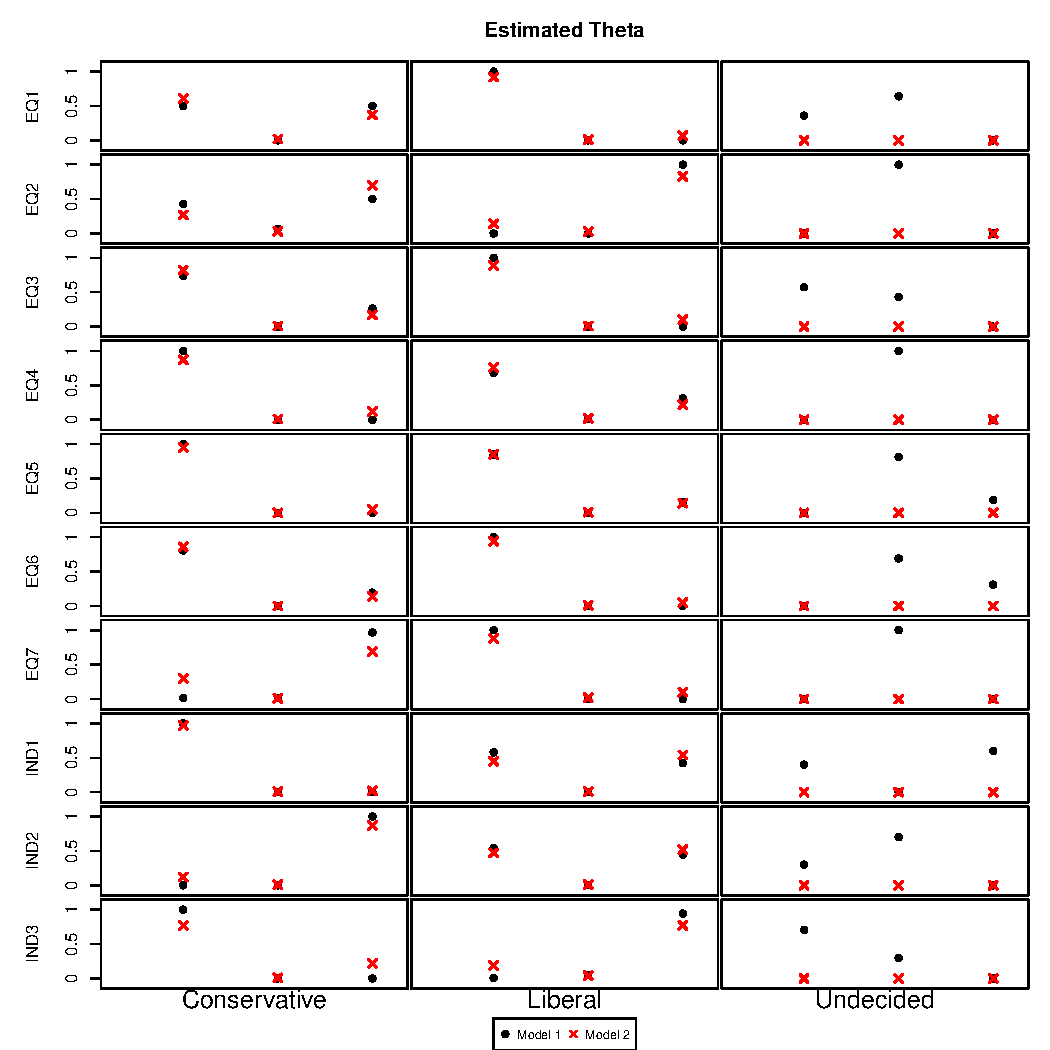
\includegraphics[width=\maxwidth]{figure/theta-1} 

}

\caption[Individuals were asked to indicate their level of agreement with 19 opinion based statements]{Individuals were asked to indicate their level of agreement with 19 opinion based statements. The fitted multinomial response probabilities for each ideology bloc to each of the first 10 statements are displayed. On the horizontal axis, 0 indicates agree, 1 indicates can't decide, and 2 indicates disagree. The estimates from our variational analysis are denoted by the dots, the Gross and Manrique-Vallier results using MCMC are shown by the red X's. Since they do not report estimates for Group 3, the Can't Decide group, those estimates are shown as 0's. The estimates for the first 10 questions are shown.}\label{fig:theta}
\end{figure}


\end{knitrout}

When examining the estimates of $\hat \theta$, we can see from Figure \ref{fig:consprop} that of the 19 variables, the statements most likely to elicit agreement from sub-population 1 are statement \texttt{IND1} (``Any person who is willing to work hard has a good chance of succeeding"), \texttt{IND3} (``Most people who don't get ahead should not blame the system; they really have only themselves to blame") and \texttt{ENT1} (``The less government gets involved with business and the economy, the better off this country will be"). Using traditional political ideology labels, sub-population 1 could be identified as the conservative bloc. In Figure \ref{fig:consprop}, bars shown in green indicate question to which sub-population 1 is more likely to agree ($\theta_{j,1,1} \geq .5$) and bars shown in red indicate questions to which the sub-population is not likely to agree.

\begin{knitrout}
\definecolor{shadecolor}{rgb}{0.969, 0.969, 0.969}\color{fgcolor}\begin{kframe}
\begin{alltt}
\hlstd{pop1VarOrder} \hlkwb{<-} \hlkwd{colnames}\hlstd{(ANES)[}\hlkwd{order}\hlstd{(out.permute}\hlopt{$}\hlstd{theta[,} \hlnum{1}\hlstd{,} \hlnum{1}\hlstd{],} \hlkwc{decreasing} \hlstd{= T)]}
\hlstd{pop1VarAgree} \hlkwb{<-} \hlkwd{sort}\hlstd{(out.permute}\hlopt{$}\hlstd{theta[,} \hlnum{1}\hlstd{,} \hlnum{1}\hlstd{],} \hlkwc{decreasing} \hlstd{= T)}
\hlkwd{barplot}\hlstd{(}\hlkwc{height} \hlstd{= pop1VarAgree,} \hlkwc{names.arg} \hlstd{= pop1VarOrder,}
        \hlkwc{main} \hlstd{=} \hlstr{"Propensity to Agree"}\hlstd{,}
        \hlkwc{cex.names} \hlstd{=} \hlnum{.7}\hlstd{,} \hlkwc{las} \hlstd{=} \hlnum{2}\hlstd{,} \hlkwc{xlab} \hlstd{=} \hlstr{"Value Statements"}\hlstd{,}
        \hlkwc{ylab} \hlstd{=} \hlkwd{expression}\hlstd{(}\hlkwd{paste}\hlstd{(theta[}\hlstr{"j,1,1"}\hlstd{])),}
        \hlkwc{col} \hlstd{=} \hlkwd{ifelse}\hlstd{(pop1VarAgree} \hlopt{>} \hlnum{.5}\hlstd{,} \hlstr{"forestgreen"}\hlstd{,} \hlstr{"darkred"}\hlstd{))}
\end{alltt}
\end{kframe}\begin{figure}

{\centering 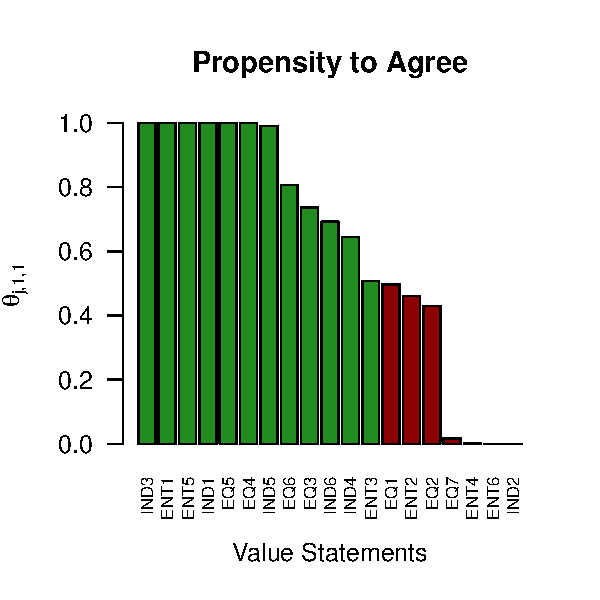
\includegraphics[width=\maxwidth]{figure/consprop-1} 

}

\caption[Propensity to agree with each opinion-based statement for the conservative bloc]{Propensity to agree with each opinion-based statement for the conservative bloc}\label{fig:consprop}
\end{figure}


\end{knitrout}

We can see from Figure \ref{fig:libprop} that for sub-population 2, the statements most likely to elicit agreement are statements \texttt{EQ7} (``One of the big problems in this country is that we don't give everyone an equal chance"), \texttt{IND6} (``Even if people try hard, they often cannot reach their goals
") and \texttt{EQ1} (``If people were treated more equally in this country, we would have many fewer problems
"). Sub-population 2 could be identified as the liberal bloc. 

\begin{knitrout}
\definecolor{shadecolor}{rgb}{0.969, 0.969, 0.969}\color{fgcolor}\begin{kframe}
\begin{alltt}
\hlstd{pop2VarOrder} \hlkwb{<-} \hlkwd{colnames}\hlstd{(ANES)[}\hlkwd{order}\hlstd{(out.permute}\hlopt{$}\hlstd{theta[,} \hlnum{2}\hlstd{,} \hlnum{1}\hlstd{],} \hlkwc{decreasing} \hlstd{= T)]}
\hlstd{pop2VarAgree} \hlkwb{<-} \hlkwd{sort}\hlstd{(out.permute}\hlopt{$}\hlstd{theta[,} \hlnum{2}\hlstd{,} \hlnum{1}\hlstd{],} \hlkwc{decreasing} \hlstd{= T)}
\hlkwd{barplot}\hlstd{(}\hlkwc{height} \hlstd{= pop2VarAgree,}
        \hlkwc{names.arg} \hlstd{= pop2VarOrder,} \hlkwc{main} \hlstd{=} \hlstr{"Propensity to Agree"}\hlstd{,}
        \hlkwc{cex.names} \hlstd{=} \hlnum{.7}\hlstd{,} \hlkwc{las} \hlstd{=} \hlnum{2}\hlstd{,} \hlkwc{xlab} \hlstd{=} \hlstr{"Value Statements"}\hlstd{,}
        \hlkwc{ylab} \hlstd{=} \hlkwd{expression}\hlstd{(}\hlkwd{paste}\hlstd{(theta[}\hlstr{"j,2,1"}\hlstd{])),}
        \hlkwc{col} \hlstd{=} \hlkwd{ifelse}\hlstd{(pop2VarAgree} \hlopt{>} \hlnum{.5}\hlstd{,} \hlstr{"forestgreen"}\hlstd{,} \hlstr{"darkred"}\hlstd{))}
\end{alltt}
\end{kframe}\begin{figure}

{\centering 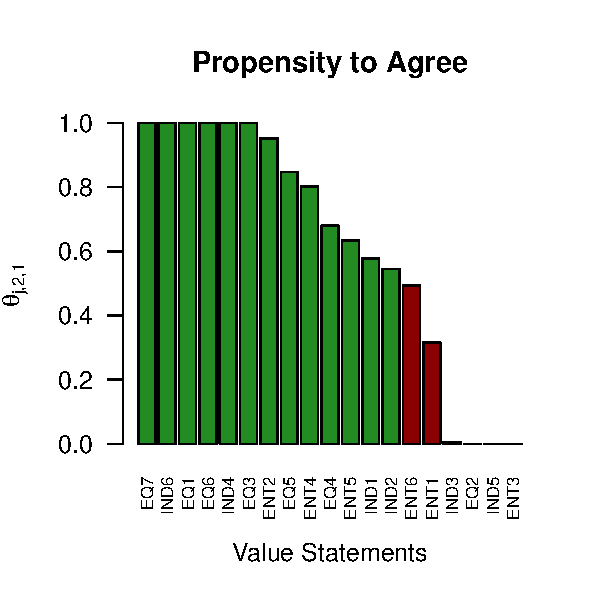
\includegraphics[width=\maxwidth]{figure/libprop-1} 

}

\caption[Propensity to agree with each opinion-based statement for the liberal bloc]{Propensity to agree with each opinion-based statement for the liberal bloc}\label{fig:libprop}
\end{figure}


\end{knitrout}

We also observe, that sub-population 3 has a much higher propensity to respond ``can't decide" then sub-populations 1 or 2. The 5 individuals with particularly large membership in group 3 responded ``can't decide" 42 times. This is particularly salient since there are only 99 ``can't decide" responses in the entire sample. Thus, sub-population 3 could be identified as the ``Can't Decide" bloc. 

\begin{knitrout}
\definecolor{shadecolor}{rgb}{0.969, 0.969, 0.969}\color{fgcolor}\begin{kframe}
\begin{alltt}
\hlcom{# Point estimates for lambda}
\hlstd{lambda.point} \hlkwb{<-} \hlstd{out.permute}\hlopt{$}\hlstd{phi} \hlopt{/} \hlkwd{rowSums}\hlstd{(out.permute}\hlopt{$}\hlstd{phi)}
\hlcom{# number of individuals which exhibit more than .3 degree of membership}
\hlcom{# in the undecided group}
\hlkwd{sum}\hlstd{(lambda.point[,} \hlnum{3}\hlstd{]} \hlopt{>=} \hlnum{.3}\hlstd{)}
\end{alltt}
\begin{verbatim}
## [1] 5
\end{verbatim}
\begin{alltt}
\hlcom{# number of can not decide responses from those with high membership in undecided group}
\hlkwd{sum}\hlstd{(ANES[}\hlkwd{which}\hlstd{(lambda.point[,} \hlnum{3}\hlstd{]} \hlopt{>=} \hlnum{.3}\hlstd{),]} \hlopt{==} \hlnum{1}\hlstd{)}
\end{alltt}
\begin{verbatim}
## [1] 42
\end{verbatim}
\end{kframe}
\end{knitrout}

\subsubsection{Interpretation of $\hat \alpha$}\label{alphaHat}
When examining the fitted value of $\hat \alpha$, we see that the conservatives and liberals are the 2 dominant groups with the undecided group comprising a much smaller portion of the population. Also, the large values of $\hat \alpha_1$ and $\hat \alpha_2$, indicate a high level of mixing between those sub-populations.  Since the estimated relative frequency of the undecided bloc is less than 1\%, we focus our interpretation on the other two blocs dominant blocs.

\begin{knitrout}
\definecolor{shadecolor}{rgb}{0.969, 0.969, 0.969}\color{fgcolor}\begin{kframe}
\begin{alltt}
\hlstd{relativeFrequency} \hlkwb{<-} \hlstd{out.permute}\hlopt{$}\hlstd{alpha} \hlopt{/} \hlkwd{sum}\hlstd{(out.permute}\hlopt{$}\hlstd{alpha)}
\end{alltt}
\end{kframe}
\end{knitrout}

% latex table generated in R 3.1.2 by xtable 1.7-4 package
% Sun Aug 16 14:52:15 2015
\begin{table}[ht]
\centering
\begin{tabular}{rrrr}
  \hline
 & Conservatives & Liberals & Undecided \\ 
  \hline
Estimated Alpha & 3.617 & 3.448 & 0.029 \\ 
  Estimate Relative Frequency & 0.510 & 0.486 & 0.004 \\ 
   \hline
\end{tabular}
\caption{Variational Estimates of Alpha} 
\end{table}


\subsubsection{Using Hellinger Distance to Determine Defining Characteristics for Each Bloc}
We might also be interested in seeing which questions are the most polarizing (the questions to which a conservative is most likely to respond differently than a liberal). These particular value statements provide insight into defining what makes a conservative and what makes a liberal. We use the Hellinger distance, a measure of the difference between distributions, to compare the conservative and liberal response probabilities for each question. Hellinger distance is defined as

\begin{equation}
H(P,Q) = \frac{1}{\sqrt{2}}\sqrt{\sum_i \left(\sqrt{p_i} - \sqrt{q_i}\right)^2}.
\end{equation}

A Hellinger distance close to 1 indicates that two probability distributions are dissimilar, while a Hellinger distance close to 0 indicates that the two probaility distirbutions are similar. We can see in Figure \ref{fig:polarizing} that the three most polarizing questions, as measured by the Hellinger distance, are statements \texttt{IND5} (``If people work hard, they almost always get what they want"), \texttt{IND3} (``Most people who don't get ahead should not blame the system; they really have only themselves to blame") and \texttt{EQ7} (``One of the big problems in this country is that we don't give everyone an equal chance"). Thus, it would seem that the most polarizing issues in 1983 revolved around access and opportunity for advancement.

\begin{knitrout}
\definecolor{shadecolor}{rgb}{0.969, 0.969, 0.969}\color{fgcolor}\begin{kframe}
\begin{alltt}
\hlstd{hellingerDist} \hlkwb{<-} \hlstd{(}\hlnum{1}\hlopt{/}\hlkwd{sqrt}\hlstd{(}\hlnum{2}\hlstd{))} \hlopt{*} \hlkwd{sqrt}\hlstd{(}\hlkwd{rowSums}\hlstd{( (}\hlkwd{sqrt}\hlstd{(out.permute}\hlopt{$}\hlstd{theta[,} \hlnum{1}\hlstd{, ])}
                                          \hlopt{-} \hlkwd{sqrt}\hlstd{(out.permute}\hlopt{$}\hlstd{theta[,} \hlnum{2}\hlstd{, ]))}\hlopt{^}\hlnum{2}\hlstd{))}
\hlkwd{barplot}\hlstd{(}\hlkwd{sort}\hlstd{(hellingerDist,} \hlkwc{decreasing} \hlstd{= T),}
        \hlkwc{names.arg} \hlstd{=} \hlkwd{colnames}\hlstd{(ANES)[}\hlkwd{order}\hlstd{(hellingerDist,} \hlkwc{decreasing} \hlstd{= T)],}
        \hlkwc{main} \hlstd{=} \hlstr{"Hellinger Distance"}\hlstd{,}
        \hlkwc{cex.names} \hlstd{=} \hlnum{.7}\hlstd{,} \hlkwc{las} \hlstd{=} \hlnum{2}\hlstd{,} \hlkwc{ylab} \hlstd{=} \hlstr{"Hellinger Distance"}\hlstd{,}
        \hlkwc{ylim} \hlstd{=} \hlkwd{c}\hlstd{(}\hlnum{0}\hlstd{,} \hlnum{1}\hlstd{))}
\hlkwd{mtext}\hlstd{(}\hlstr{"Between Conservatives and Liberals"}\hlstd{)}
\end{alltt}
\end{kframe}\begin{figure}

{\centering 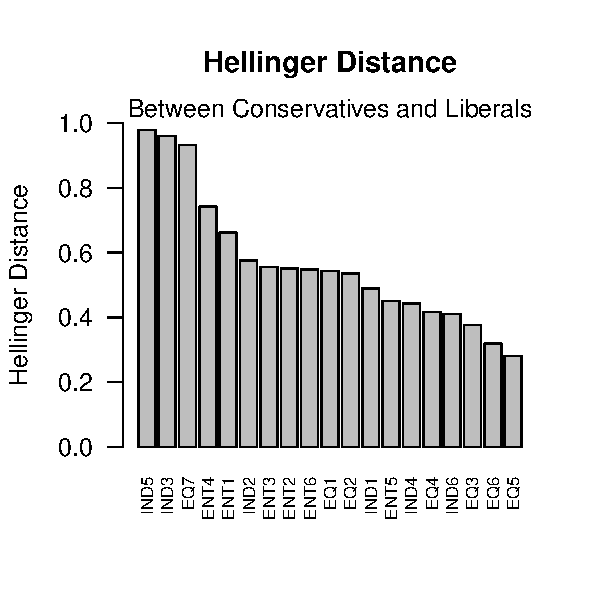
\includegraphics[width=\maxwidth]{figure/polarizing-1} 

}

\caption[Using Hellinger distance indicates that the most polarizing statements are IND 5, IND 3, and EQ 7]{Using Hellinger distance indicates that the most polarizing statements are IND 5, IND 3, and EQ 7. These were all issues involving opportunity for advancement}\label{fig:polarizing}
\end{figure}

\begin{kframe}\begin{alltt}
\hlkwd{colnames}\hlstd{(ANES)[}\hlkwd{order}\hlstd{(hellingerDist,} \hlkwc{decreasing} \hlstd{= T)][}\hlnum{1}\hlopt{:}\hlnum{3}\hlstd{]}
\end{alltt}
\begin{verbatim}
## [1] "IND5" "IND3" "EQ7"
\end{verbatim}
\end{kframe}
\end{knitrout}

\subsection{Visualizing Group Dispersion}

For the groups memberships for individuals, we use the posterior mean, $\frac{\hat \phi_i}{\sum_k \hat \phi_{i,k}}$ as point estimates for $\lambda_i$. Plotting the poster mean of each individual in Figure \ref{fig:mems}, we can see a fair amount of intra-individual mixing. 139 out of the 279 individuals have estimated memberships of at least 40\% in both the conservative and liberal blocs. This is not particularly uprising since we observed relatively large values of $\hat \alpha_1$ and $\hat \alpha_2$.
\begin{knitrout}
\definecolor{shadecolor}{rgb}{0.969, 0.969, 0.969}\color{fgcolor}\begin{kframe}
\begin{alltt}
\hlcom{# number of individuals with at least 40% membership in}
\hlcom{# both conservative and liberal blocs}
\hlkwd{sum}\hlstd{( (lambda.point[,} \hlnum{1}\hlstd{]} \hlopt{>} \hlnum{.4}\hlstd{)} \hlopt{&} \hlstd{(lambda.point[,} \hlnum{2}\hlstd{]} \hlopt{>} \hlnum{.4}\hlstd{))}
\end{alltt}
\begin{verbatim}
## [1] 139
\end{verbatim}
\end{kframe}
\end{knitrout}

\begin{knitrout}
\definecolor{shadecolor}{rgb}{0.969, 0.969, 0.969}\color{fgcolor}\begin{kframe}
\begin{alltt}
\hlkwd{plot}\hlstd{(out.permute,} \hlkwc{type} \hlstd{=} \hlstr{"membership"}\hlstd{,} \hlkwc{indices} \hlstd{=} \hlkwd{c}\hlstd{(}\hlnum{1}\hlopt{:}\hlnum{20}\hlstd{),} \hlkwc{nrow} \hlstd{=} \hlnum{5}\hlstd{,} \hlkwc{ncol} \hlstd{=} \hlnum{4}\hlstd{,} \hlkwc{main} \hlstd{=} \hlstr{"Estimated Memberships"}\hlstd{,}
     \hlkwc{groupNames} \hlstd{=} \hlkwd{c}\hlstd{(}\hlstr{"Cons"}\hlstd{,} \hlstr{"Lib"}\hlstd{,} \hlstr{"Cant Decide"}\hlstd{),} \hlkwc{fitNames} \hlstd{=} \hlkwd{c}\hlstd{(}\hlstr{"mixedMem"}\hlstd{))}
\end{alltt}
\end{kframe}\begin{figure}

{\centering 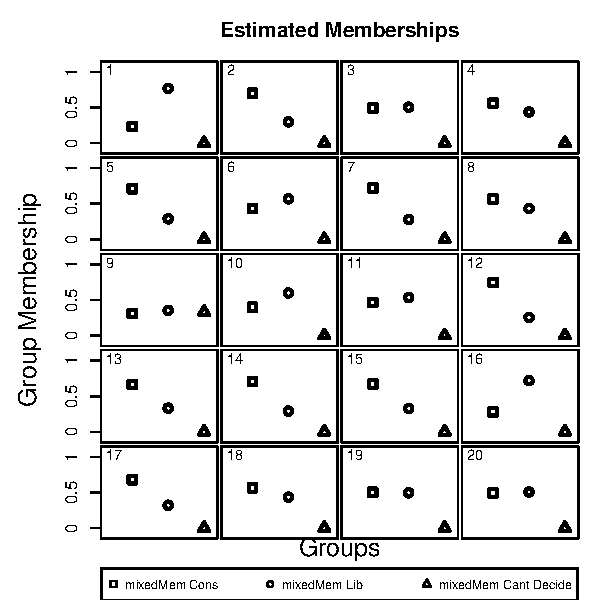
\includegraphics[width=\maxwidth]{figure/mems-1} 

}

\caption[Estimated memberships for first 42 individuals]{Estimated memberships for first 42 individuals}\label{fig:mems}
\end{figure}


\end{knitrout}
We can also plot the ``empirical CDF" of estimated membership in conservative bloc as shown in Figure \ref{fig:posteriorMem}. Since the marginal distribution of a Dirichlet distribution is a Beta distribution, we can also plot the 95\% credible intervals for the posterior membership in the conservative bloc. We observe that there is still a relatively large amount of uncertainty in the estimated membership of each individual.


\begin{knitrout}
\definecolor{shadecolor}{rgb}{0.969, 0.969, 0.969}\color{fgcolor}\begin{kframe}
\begin{alltt}
\hlstd{index} \hlkwb{<-} \hlkwd{order}\hlstd{(lambda.point[,} \hlnum{1}\hlstd{])}

\hlcom{# variance of posterior membership in conservative bloc}
\hlstd{var.Mem} \hlkwb{<-} \hlstd{out.permute}\hlopt{$}\hlstd{phi[,} \hlnum{1}\hlstd{]} \hlopt{*} \hlstd{(}\hlkwd{rowSums}\hlstd{(out.permute}\hlopt{$}\hlstd{phi)} \hlopt{-}
                                 \hlstd{out.permute}\hlopt{$}\hlstd{phi[,} \hlnum{1}\hlstd{])} \hlopt{/}
  \hlstd{(}\hlkwd{rowSums}\hlstd{(out.permute}\hlopt{$}\hlstd{phi)}\hlopt{^}\hlnum{2} \hlopt{*} \hlstd{(}\hlkwd{rowSums}\hlstd{(out.permute}\hlopt{$}\hlstd{phi)} \hlopt{+} \hlnum{1}\hlstd{))}
\hlcom{# plot posterior means}
\hlkwd{plot}\hlstd{(}\hlkwd{sort}\hlstd{(lambda.point[,} \hlnum{1}\hlstd{]),} \hlkwc{pch} \hlstd{=} \hlnum{19}\hlstd{,}
     \hlkwc{main} \hlstd{=} \hlstr{"Posterior Membership in Conservative Bloc"}\hlstd{,}
     \hlkwc{ylab} \hlstd{=} \hlstr{"Posterior Membership"}\hlstd{,} \hlkwc{xlab} \hlstd{=} \hlstr{"Individual"}\hlstd{,}
     \hlkwc{cex} \hlstd{=} \hlnum{.8}\hlstd{,} \hlkwc{ylim} \hlstd{=} \hlkwd{c}\hlstd{(}\hlnum{0}\hlstd{,} \hlnum{1}\hlstd{))}

\hlcom{# marginal distirbution of Dirichlet, is Beta distribution, so we can get posterior CI}
\hlcom{# plot posterior 90% CI}
\hlstd{ci_up} \hlkwb{<-} \hlkwd{qbeta}\hlstd{(}\hlnum{.975}\hlstd{, out.permute}\hlopt{$}\hlstd{phi[index,} \hlnum{1}\hlstd{],} \hlkwd{rowSums}\hlstd{(out.permute}\hlopt{$}\hlstd{phi[index,} \hlkwd{c}\hlstd{(}\hlnum{2}\hlopt{:}\hlnum{3}\hlstd{)]))}
\hlstd{ci_low} \hlkwb{<-} \hlkwd{qbeta}\hlstd{(}\hlnum{.025}\hlstd{, out.permute}\hlopt{$}\hlstd{phi[index,} \hlnum{1}\hlstd{],} \hlkwd{rowSums}\hlstd{(out.permute}\hlopt{$}\hlstd{phi[index,} \hlkwd{c}\hlstd{(}\hlnum{2}\hlopt{:}\hlnum{3}\hlstd{)]))}
\hlkwd{segments}\hlstd{(}\hlkwc{x0} \hlstd{=} \hlkwd{c}\hlstd{(}\hlnum{1}\hlopt{:}\hlstd{out}\hlopt{$}\hlstd{Total),} \hlkwc{y0} \hlstd{= ci_up,} \hlkwc{y1} \hlstd{= ci_low,} \hlkwc{col} \hlstd{=} \hlstr{"gray"}\hlstd{,} \hlkwc{lwd} \hlstd{=} \hlnum{.3}\hlstd{,} \hlkwc{lty} \hlstd{=} \hlnum{1}\hlstd{)}
\hlkwd{legend}\hlstd{(}\hlstr{"bottomright"}\hlstd{,} \hlkwc{legend} \hlstd{=} \hlkwd{c}\hlstd{(}\hlstr{"posterior mean"}\hlstd{,} \hlstr{"95% CI"}\hlstd{),} \hlkwc{pch} \hlstd{=} \hlkwd{c}\hlstd{(}\hlnum{19}\hlstd{,} \hlnum{NA}\hlstd{),}
       \hlkwc{lty} \hlstd{=} \hlkwd{c}\hlstd{(}\hlnum{NA}\hlstd{,} \hlnum{1}\hlstd{),} \hlkwc{col} \hlstd{=} \hlkwd{c}\hlstd{(}\hlstr{"black"}\hlstd{,} \hlstr{"gray"}\hlstd{))}
\end{alltt}
\end{kframe}\begin{figure}

{\centering 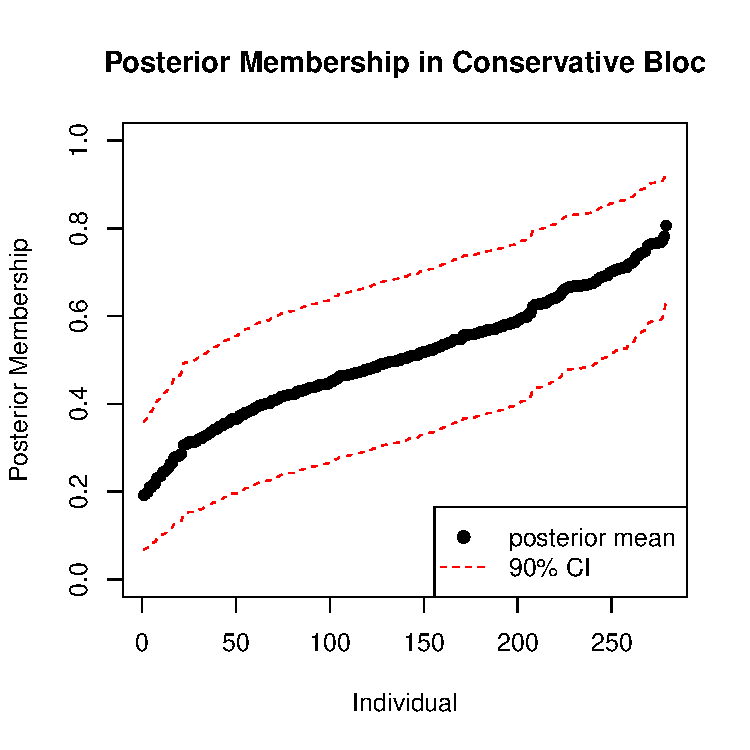
\includegraphics[width=\maxwidth]{figure/posteriorMem-1} 

}

\caption[We observe a relatively high rate of intra-individual mixing]{We observe a relatively high rate of intra-individual mixing}\label{fig:posteriorMem}
\end{figure}


\end{knitrout}


\subsection{Comparison of MCMC and Variational Results}
Comparing the results of the MCMC analysis by \cite{grossManriqueVallier} to the results from our variational analysis, we see they are very similar. In both analyses, we identify two dominant profiles- a conservative bloc and a liberal bloc- as well as a much smaller undecided faction. As can be seen in Figure 2, the variational estimates of $\theta$ agree well with the MCMC estimates.

Since Gross and Manrique-Vallier utilize a fully Bayesian specification, they  are able to utilize a hypothesis testing framework with $\theta$ to find the most polarizing issues. Because the variational analysis only provides point estimates of $\theta$, we used Hellinger distances instead. However, both analyses agree that the three most polarizing statements are  \texttt{IND5}, \texttt{IND3} and \texttt{EQ7}.

Although the broad interpretation and estimates of $\theta$ agree, we do see differences in the estimates of $\alpha$. Gross and Manrique-Vallier report a posterior mean of $\alpha = \left(0.462, 0.285, 0.01 8\right)$ yielding relative frequencies of $\left(60.4\%, 37.3\%, 2.3\%\right)$ for the conservative, liberal and undecided bloc respectively. Although MCMC ordering of the relative frequency matches the ordering of the variational estimates, this implies a much lower level of intra-individual mixing and as well as a higher relative frequency for the conservative bloc.

\section{Conclusion} \label{conclusion}
In this tutorial, we only briefly introduced the ideas of mixed membership models. For more interested readers, \cite{Airoldi2014Handbook} provide a much deeper exposition of mixed membership models as well as a variety of different applications. 

We also provide a step-by-step guide for using \texttt{mixedMem} as well as some sample visualizations/interpretations which may be helpful to the user. From the political survey example, we see that the use of variational inference largely agrees with the more complicated MCMC procedure, and still provides reasonable and interpretable results.

By providing an R package for fitting mixed membership models, we aim to aid researchers who are studying problems where a mixed membership analysis is compelling, but have been otherwise dissuaded by the computational difficulties. We hope that this package extends the use of mixed membership models to a variety of new disciplines and interesting scientific problems.

\bibliographystyle{plainnat}
\bibliography{pl}

\end{document}
